\documentclass{article}

% NeurIPS 2026 style
\usepackage[final]{neurips_2026}

\usepackage[utf8]{inputenc}
\usepackage[T1]{fontenc}
\usepackage{hyperref}
\usepackage{url}
\usepackage{booktabs}
\usepackage{amsfonts}
\usepackage{amsmath}
\usepackage{amssymb}
\usepackage{nicefrac}
\usepackage{microtype}
\usepackage{graphicx}
\usepackage{xcolor}
\usepackage{algorithm}
\usepackage{algorithmic}
\usepackage{subcaption}
\usepackage{multirow}
\usepackage{wrapfig}

\graphicspath{{figures/}{../outputs/standard/analysis/}{../outputs/vla/}}

\newcommand{\attnres}{\textsc{AttnRes}}
\newcommand{\reskip}{\textsc{ReSkip}}
\newcommand{\reloop}{\textsc{ReLoop}}
\newcommand{\E}{\mathbb{E}}
\newcommand{\R}{\mathbb{R}}
\newcommand{\softmax}{\text{softmax}}

\title{Attention Residuals as Adaptive Computation Routers: \\
Input-Dependent Depth for LLMs and Vision-Language-Action Models}

\author{
  Author One\thanks{Equal contribution.} \\
  Affiliation \\
  \texttt{email@example.com} \\
  \And
  Author Two\footnotemark[1] \\
  Affiliation \\
  \texttt{email@example.com} \\
}

\begin{document}

\maketitle

\begin{abstract}
We propose using Attention Residuals (\attnres{})---learned, input-dependent weighted combinations over transformer depth---as zero-cost routing signals for adaptive computation.
While standard residual connections treat all layers equally, \attnres{} learns softmax attention weights $\alpha_{n \to l}$ over previous block outputs, exposing an importance map over the depth dimension.
Crucially, \attnres{} block execution is naturally two-phase---a phase-1 attention over already-completed blocks occurs \emph{before} each block runs---making its routing statistics available as a pre-execution decision signal at near-zero cost.
We show that these signals directly guide two forms of adaptive computation:
(1)~\reskip{}, which makes per-input, per-position skip decisions from phase-1 statistics and uses position-calibrated thresholds to protect quality;
on a 340M transformer trained on FineWeb-Edu, \reskip{} achieves \textbf{$1.19\times$ wall-clock speedup} with \textbf{zero degradation} across LAMBADA, HellaSwag, ARC-Easy, and ARC-Challenge.
We further identify an important disconnect between \emph{AttnRes importance} (how often a block is referenced) and \emph{ablation impact} (whether it is irreplaceable), and show that combining ablation-informed with importance-informed position selection yields strictly better Pareto fronts than using either signal alone.
(2)~\reloop{} uses $K$ weight-shared blocks applied a variable number of times, where \attnres{} pseudo-queries differentiate each application's role despite shared weights.
For Vision-Language-Action (VLA) models, \attnres{} naturally discovers modality-specific depth utilization, enabling modality-aware skipping for robotics inference without sacrificing manipulation success rates.
Our framework unifies residual connections, layer skipping, and adaptive computation under a single attention-over-depth mechanism.
\end{abstract}

%----------------------------------------------------------------------
\section{Introduction}
\label{sec:intro}
%----------------------------------------------------------------------

Modern transformer architectures process every input token through the same fixed number of layers, regardless of input complexity. This uniform computation is wasteful: simple inputs (factual recall, syntactic pattern matching) may need only shallow processing, while complex inputs (multi-step reasoning, compositional planning) require deep iterative refinement~\citep{graves2016adaptive, dehghani2018universal}.

Several lines of work address this inefficiency. \textit{Early exit} methods~\citep{schuster2022confident, elbayad2020depth} add auxiliary classifiers at each layer to decide when to stop. \textit{Layer pruning}~\citep{gromov2024unreasonable, men2024shortgpt} removes entire layers post-hoc based on importance metrics. \textit{Mixture-of-Depths}~\citep{raposo2024mixture} learns per-token routing during training with auxiliary capacity losses. \textit{Universal Transformers}~\citep{dehghani2018universal} share weights across depth but struggle to differentiate the role of each application of the same block.

All these methods share a common limitation: they require \emph{additional} mechanisms---exit classifiers, importance estimators, routing networks, or auxiliary losses---that are external to the core transformer computation. This creates a fundamental tension: the routing signal is learned separately from the representations it routes.

\textbf{Our key insight} is that Attention Residuals~\citep{chen2026attnres}, which replace fixed residual connections with learned attention over the depth dimension, \emph{already provide} the routing signal needed for adaptive computation. The \attnres{} mechanism learns input-dependent weights $\alpha_{i \to l}$ that determine how much each layer~$l$ attends to each previous layer~$i$'s output. These weights are:
\begin{enumerate}
    \item \textbf{Input-dependent}: Different inputs produce different depth-wise attention patterns
    \item \textbf{Decoupled from forward computation}: The pseudo-query $\mathbf{w}_l$ can be evaluated before executing layer~$l$
    \item \textbf{Competitively normalized}: Softmax creates explicit ``unimportant'' signals
    \item \textbf{Already learned}: No auxiliary losses or additional parameters beyond the \attnres{} mechanism itself
\end{enumerate}

We exploit these properties to propose two adaptive computation strategies:

\textbf{\reskip{}} (Section~\ref{sec:reskip}): At inference time, we read phase-1 \attnres{} statistics---available \emph{before} each block executes---and make per-input skip decisions against position-calibrated thresholds. Because the two-phase execution is intrinsic to \attnres{}, the skip decision adds no architectural change and no auxiliary network. On a 340M model we preserve full-depth scores on all four benchmarks at $1.19\times$ wall-clock speedup, and we identify a principled way to combine ablation-informed and importance-informed position selection that dominates either signal used alone.

\textbf{\reloop{}} (Section~\ref{sec:reloop}): We maintain $K$ weight-shared blocks applied up to $M$ times each, where \attnres{} pseudo-queries are unique per depth \emph{position} (not per block). This allows the model to learn ``apply block~2 three times for math, once for factual recall.'' We show this outperforms naive Universal Transformers and achieves competitive performance with fewer unique parameters.

\textbf{VLA Adaptive Depth} (Section~\ref{sec:vla}): For Vision-Language-Action models, we show that \attnres{} naturally discovers modality-specific depth patterns without explicit supervision. Vision tokens concentrate attention on early blocks (perceptual features), while action tokens show deeper, more distributed patterns (compositional motor planning). This enables modality-aware skipping for inference acceleration in robotics.

%----------------------------------------------------------------------
\section{Background: Attention Residuals}
\label{sec:background}
%----------------------------------------------------------------------

\subsection{Standard Residual Connections}

In a standard transformer with $L$ layers, the output of layer $l$ is:
\begin{equation}
    \mathbf{x}_l = \mathbf{x}_{l-1} + f_l(\mathbf{x}_{l-1})
\end{equation}
where $f_l$ is the layer function (attention + FFN). Unrolling the recursion:
\begin{equation}
    \mathbf{x}_L = \mathbf{x}_0 + \sum_{l=1}^{L} f_l(\mathbf{x}_{l-1})
\end{equation}
This is a \emph{fixed, uniform} combination---every layer's contribution has equal weight of~1, regardless of the input.

\subsection{Attention Residuals}

\attnres{}~\citep{chen2026attnres} replaces the fixed residual with a \emph{learned attention over depth}. Each layer $l$ has a pseudo-query $\mathbf{w}_l \in \R^d$ that attends over all previous layer outputs $\{\mathbf{h}_0, \ldots, \mathbf{h}_{l-1}\}$:
\begin{equation}
    \alpha_{i \to l} = \frac{\exp(\mathbf{w}_l^\top \mathbf{k}_i / \sqrt{d})}{\sum_{j=0}^{l-1} \exp(\mathbf{w}_l^\top \mathbf{k}_j / \sqrt{d})}
    \label{eq:attnres_weights}
\end{equation}
\begin{equation}
    \mathbf{x}_l = \sum_{i=0}^{l-1} \alpha_{i \to l} \cdot \mathbf{h}_i
    \label{eq:attnres_combine}
\end{equation}
where $\mathbf{k}_i = W_K \mathbf{h}_i$ is the key projection of layer $i$'s output, and $\mathbf{h}_i$ denotes the output of layer $i$ \emph{after} applying $f_i$.

\textbf{Block \attnres{}} groups layers into $N$ blocks and applies the attention mechanism at the block level, providing coarser-grained routing suitable for skip/loop decisions.

\textbf{Online softmax merge} (Algorithm~\ref{alg:online_merge}) enables memory-efficient computation by incrementally updating the weighted combination as each layer produces output, without storing all previous outputs simultaneously.

\begin{algorithm}[t]
\caption{Two-phase \attnres{} forward with dynamic \reskip{}}
\label{alg:online_merge}
\begin{algorithmic}[1]
\STATE \textbf{Input:} Embeddings $\mathbf{h}_0$; block functions $f_1, \ldots, f_N$; \attnres{} routers $\{\mathbf{w}_n\}$; eligible positions $\mathcal{P}$; thresholds $\{\tau_n\}_{n\in\mathcal{P}}$; max skips $M_{\max}$.
\STATE Initialize online-softmax state $(\mathbf{s}, m, e)$ from $\mathbf{h}_0$;\ \ skip counter $k\gets 0$.
\FOR{$n = 1$ to $N$}
    \STATE \textbf{Phase 1 (probe):} compute $\alpha_{\cdot \to n}$ over completed block outputs $\{\mathbf{h}_0, \ldots, \mathbf{h}_{n-1}\}$ and the running state $(\mathbf{s}, m, e)$.
    \STATE Extract $w_{\text{recent}}(n) \gets \E_{\text{token}}[\alpha_{n-1 \to n}]$.
    \IF{$n \in \mathcal{P}$ \textbf{and} $k < M_{\max}$ \textbf{and} $w_{\text{recent}}(n) > \tau_n$}
        \STATE \textbf{Skip}: keep $(\mathbf{s}, m, e)$ unchanged, $\mathbf{h}_n \gets \mathbf{h}_{n-1}$, $k \gets k + 1$.
    \ELSE
        \STATE \textbf{Execute} block $n$: run $f_n$ on the phase-1 merged input, update $(\mathbf{s}, m, e)$ online with the new output $\mathbf{h}_n$.
    \ENDIF
\ENDFOR
\STATE \textbf{Output:} final hidden state $\mathbf{s}/e$.
\end{algorithmic}
\end{algorithm}

%----------------------------------------------------------------------
\section{\reskip{}: AttnRes-Guided Layer Skipping}
\label{sec:reskip}
%----------------------------------------------------------------------

\subsection{Motivation and two-phase execution}

\citet{gromov2024unreasonable} showed that a significant fraction of transformer layers can be pruned with minimal performance loss. \citet{chen2026attnres} observed that \attnres{} weights are highly concentrated: most layers attend overwhelmingly to their immediate predecessor and the embedding, with sparse off-diagonal connections. We go one step further and observe that \attnres{} block execution is \emph{naturally two-phase}: before block~$n$ runs, the model already computes attention over all previously completed block outputs $\{\mathbf{h}_0, \ldots, \mathbf{h}_{n-1}\}$ to form the block's input. This means the per-input routing statistics $\alpha_{\cdot \to n}$ are available \emph{as a pre-execution signal}, at near-zero additional cost. We exploit this structure to make a per-input skip decision for each block without any auxiliary classifier or training loss.

\subsection{Method}
\label{sec:reskip_method}

\paragraph{Block importance and ablation impact (offline statistics).}
For a trained model we characterise each block~$n$ with two complementary scores computed on a calibration set:
\begin{align}
    I(n) &= \max_{l > n}\,\E\big[\alpha_{n \to l}\big] && \text{(\emph{AttnRes importance}: how often block $n$ is referenced downstream)} \label{eq:importance}\\
    A(n) &= \frac{\text{PPL}(\text{model with block $n$ statically removed})}{\text{PPL}(\text{full-depth})} && \text{(\emph{ablation impact}: is block $n$ irreplaceable?)} \label{eq:ablation}
\end{align}
These two scores are related but \emph{not monotonic}; their disagreement turns out to be crucial (Section~\ref{sec:reskip_finding}).

\paragraph{Dynamic skip from phase-1 statistics.}
At inference, for each block position~$n$ we inspect the phase-1 attention weights over already-completed blocks. Let $w_{\text{recent}}(n)$ denote the mean weight (over tokens in the batch) that position~$n$'s router places on the \emph{most recently executed} block. Our default policy is \texttt{recent\_weight\_gt}:
\begin{equation}
    \text{skip block } n \iff w_{\text{recent}}(n) > \tau_n \quad\text{and}\quad n \in \mathcal{P},\quad \textstyle\sum_{m<n}\mathbb{1}[\text{skipped}_m] < M_{\max}.
    \label{eq:skip_rule}
\end{equation}
Here $\mathcal{P}$ is a set of \emph{eligible positions} (see below) and $M_{\max}$ caps the number of skips per forward pass. Intuitively, if the next-block router already indicates it wants to copy the most recent output, block~$n$ is doing local refinement that we can safely drop.

\paragraph{Position-specific calibrated thresholds.}
A single global $\tau$ is sub-optimal: different positions produce different distributions of $w_{\text{recent}}$. We calibrate per position on a held-out set of 32 long-context sequences, setting $\tau_n$ to the $q$-th empirical quantile of $w_{\text{recent}}(n)$ (we use $q{=}0.85$ by default). This yields stronger accuracy--compute Pareto points than any single global threshold.

\paragraph{Eligible-position selection using \emph{two} signals.}
Naively setting $\mathcal{P}$ to all interior positions is too aggressive---our sweeps show this forces PPL ratios above 1.3 even at mild quantiles (Figure~\ref{fig:reskip_pareto}). Prior work (including early versions of this system) picks $\mathcal{P}$ by low $I(n)$ alone. We argue that \emph{both} signals matter:
\begin{itemize}
    \item \textbf{Low $I(n)$} $\Rightarrow$ skip triggers \emph{frequently}: the next block genuinely rarely uses this block's output.
    \item \textbf{Low $A(n)$} $\Rightarrow$ skip is \emph{safe}: even if triggered on a non-trivial input, quality is preserved.
\end{itemize}
The two signals favor different blocks and together define a cleaner candidate set than either alone.

\paragraph{Implementation.}
The full decision adds a phase-1 probe (one attention head over $n$ completed blocks, no MLP) before each eligible block, reads $w_{\text{recent}}(n)$, compares to $\tau_n$, and either skips (excluding the block from the online softmax merge, Algorithm~\ref{alg:online_merge}) or executes normally. No architectural changes, no additional parameters, no training modifications. The calibration step---a single 32-batch pass over held-out data---produces $\tau_n$ and can be embedded into the exported checkpoint's \texttt{config.json}, so downstream users simply load and run.

\textbf{Key advantages over existing methods:}
\begin{itemize}
    \item \textbf{vs.\ CALM}~\citep{schuster2022confident}: No auxiliary exit classifiers needed.
    \item \textbf{vs.\ Mixture-of-Depths}~\citep{raposo2024mixture}: No per-token routing or capacity losses during training.
    \item \textbf{vs.\ Static pruning}~\citep{gromov2024unreasonable}: Input-dependent per-batch decisions, not a fixed keep-mask.
    \item \textbf{vs.\ LayerSkip}~\citep{elhoushi2024layerskip}: No self-speculative decoding overhead.
\end{itemize}

\subsection{Experimental setup}
\label{sec:reskip_setup}

\textbf{Model.} We use a Block \attnres{} transformer with $d_{\text{model}}{=}1024$, $L{=}24$ layers grouped into $N{=}8$ blocks (${\sim}340$M parameters), SwiGLU FFN, RoPE positional embeddings, and a 32k vocabulary.

\textbf{Data.} Pretrained on FineWeb-Edu~100BT~\citep{penedo2024fineweb} with streaming and variable-length packing; we use the public tokenizer and train for 35k steps at sequence length 32k with gradient accumulation. Training does not involve any skip signal.

\textbf{Calibration and evaluation.} We calibrate $\tau_n$ on 32 held-out sequences of length 8192. For wall-clock measurements we use 48 cached sequences (4 warmup, 44 measured) of length 8192 on a single H100; for downstream quality we report \texttt{lm-eval-harness}~\citep{eval-harness} results on LAMBADA~\citep{paperno2016lambada}, HellaSwag~\citep{zellers2019hellaswag}, ARC-Easy and ARC-Challenge~\citep{clark2018arc}.

\subsection{The importance--ablation disconnect}
\label{sec:reskip_finding}

Figure~\ref{fig:reskip_routing}(a) visualises the learned \attnres{} routing weights for our 340M model. Most blocks concentrate on their immediate predecessor, with sparse long-range attention to the embedding and the final block; \textit{I(n)} is highest for intermediate blocks and lowest for the first and last interior blocks, as expected.

\begin{figure}[t]
    \centering
    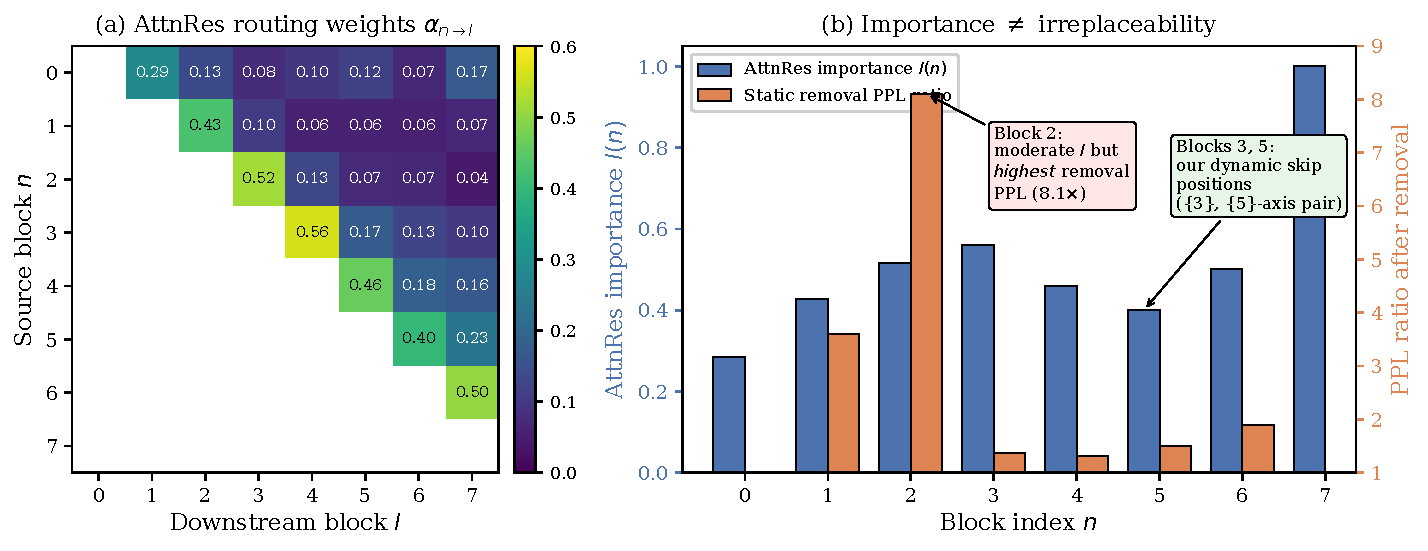
\includegraphics[width=\textwidth]{reskip_routing_importance_vs_ablation.pdf}
    \caption{\textbf{AttnRes routing weights do not predict ablation impact (340M).}
    (a)~Learned block-level attention $\alpha_{n \to l}$. (b)~Per-block \emph{AttnRes importance} $I(n)$ (blue, left axis) and \emph{static removal PPL ratio} $A(n)$ (orange, right axis). Block~2 has moderate $I$ yet the highest removal impact ($8.1\times$ PPL); blocks~3--5 span the space of low ablation impact but with very different importance levels. Dynamic skip needs \emph{both} signals: low $I$ to trigger often and low $A$ to trigger safely.}
    \label{fig:reskip_routing}
\end{figure}

\begin{wraptable}{r}{0.45\textwidth}
\vspace{-4pt}
\centering
\footnotesize
\caption{Dynamic skip as a function of the candidate position set $\mathcal{P}$ on 340M (seq\_len=8192, $M_{\max}{=}2$, $q{=}0.85$). A single position ($\mathcal{P}{=}\{5\}$) or naive aggressive sets ($\mathcal{P}{=}\{2,3,\ldots,6\}$) are dominated by our combined choice.}
\label{tab:reskip_position_ablation}
\begin{tabular}{lcc}
\toprule
$\mathcal{P}$ & PPL ratio & Speedup \\
\midrule
$\{5\}$ ($I$-only) & 0.993 & 1.14$\times$ \\
$\{3\}$ ($A$-only) & 1.009 & 1.02$\times$ \\
$\{2,3\}$ & 1.009 & 1.17$\times$ \\
$\{4,5\}$ & 1.008 & 0.97$\times$ \\
$\{3,4,5\}$ & 0.993 & 1.02$\times$ \\
$\{2,3,4,5,6\}$ & 1.40 & 1.16$\times$ \\
\midrule
\textbf{$\{3,5\}$ (ours)} & \textbf{0.991} & \textbf{1.19$\times$} \\
\bottomrule
\end{tabular}
\vspace{-12pt}
\end{wraptable}

The striking observation in Figure~\ref{fig:reskip_routing}(b) is that $I(n)$ and the static ablation PPL $A(n)$ \emph{disagree on a case-by-case basis}. Block~2 has middle-of-the-pack importance ($I{=}0.52$) but is \emph{catastrophic} to remove (${A{=}8.1\times}$). Block~4 has the single \emph{lowest} static ablation impact (${A{=}1.31\times}$) yet a higher importance than block~5 and---as we show below---is not a productive dynamic skip target. The most effective dynamic-skip positions are those that score well on \emph{both} axes: block~5 (lowest $I$ and moderate $A$) and block~3 (moderately high $I$ but close to the lowest $A$).

Table~\ref{tab:reskip_position_ablation} quantifies this on our 340M model. Using block~5 alone (the low-$I$ choice favored by prior work) yields $1.14\times$; using block~3 alone (low-$A$) is essentially a no-op because the phase-1 router almost never triggers on block~3. Combining them---our default $\mathcal{P}{=}\{3,5\}$ with $M_{\max}{=}2$---achieves $1.19\times$ with PPL slightly \emph{below} full-depth on the proxy set. Importantly, block~4's low $A$ does \emph{not} transfer to dynamic skip: it has moderate $I$ and its phase-1 trigger rate is low, so trying to force it into the set simply adds probe cost.

\subsection{Results}
\label{sec:reskip_results}

\begin{table}[t]
\caption{Downstream benchmark comparison on 340M FineWeb-Edu. Dynamic \reskip{} preserves every metric bit-for-bit while running $1.19\times$ faster end-to-end at sequence length 8192.}
\label{tab:reskip_benchmark}
\centering
\begin{tabular}{lccccc}
\toprule
\textbf{Configuration} & \textbf{LAMBADA acc} & \textbf{LAMBADA ppl} & \textbf{HellaSwag} & \textbf{ARC-E} & \textbf{ARC-C} \\
\midrule
Full-depth & 0.4056 & 20.20 & 0.4607 & 0.5438 & 0.3012 \\
\reskip{} ($\mathcal{P}{=}\{5\}, M_{\max}{=}1, q{=}0.95$) & \textbf{0.4056} & \textbf{20.20} & \textbf{0.4607} & \textbf{0.5438} & \textbf{0.3012} \\
\reskip{} ($\mathcal{P}{=}\{3,5\}, M_{\max}{=}2, q{=}0.85$) & \textbf{0.4056} & \textbf{20.20} & \textbf{0.4607} & \textbf{0.5438} & \textbf{0.3012} \\
\bottomrule
\end{tabular}
\end{table}

\begin{figure}[t]
    \centering
    \begin{subfigure}[b]{0.55\textwidth}
        \centering
        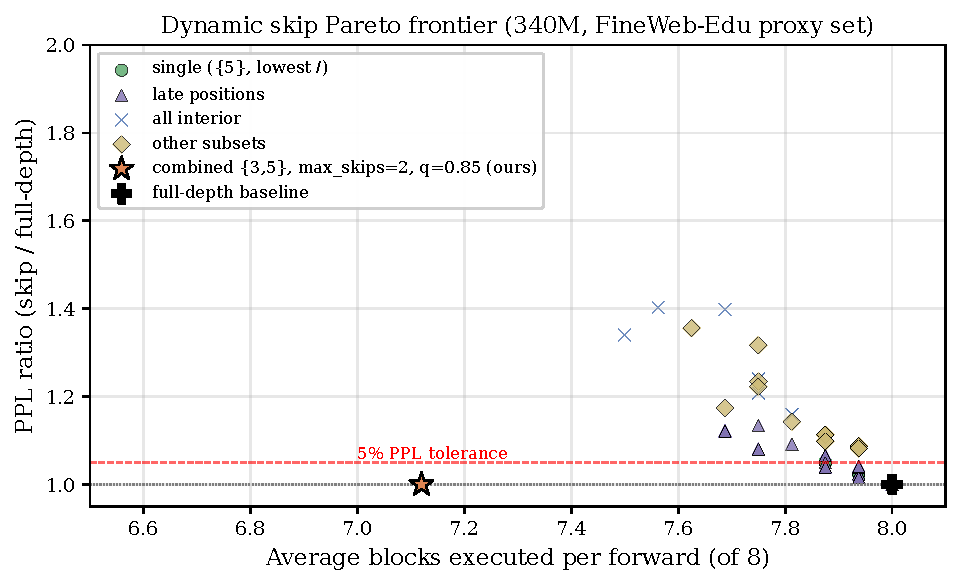
\includegraphics[width=\textwidth]{reskip_pareto.pdf}
        \caption{Accuracy--compute Pareto. Our combined position set (orange star) sits strictly below the 5\% PPL tolerance while using the fewest blocks among safe configurations.}
        \label{fig:reskip_pareto}
    \end{subfigure}
    \hfill
    \begin{subfigure}[b]{0.42\textwidth}
        \centering
        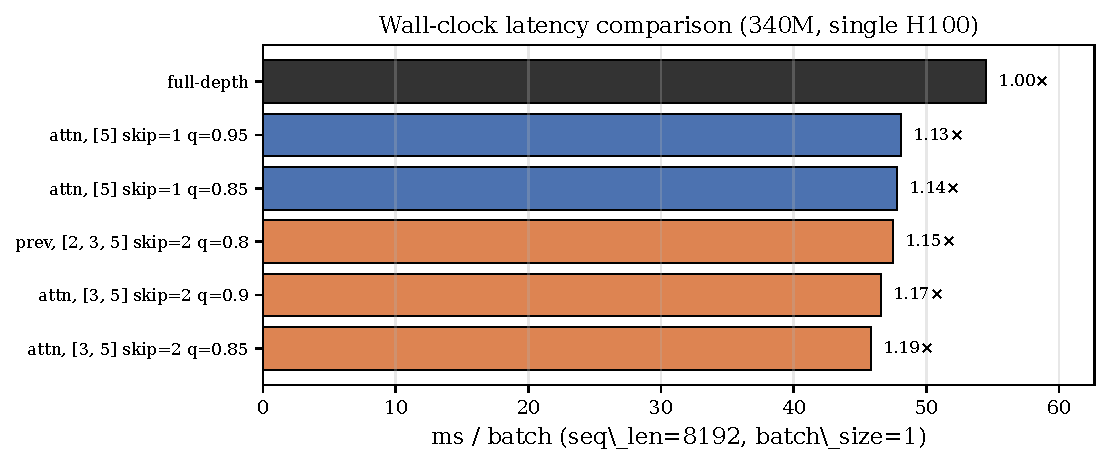
\includegraphics[width=\textwidth]{reskip_latency.pdf}
        \caption{Wall-clock latency on a single H100 at seq\_len=8192. Moving from $\{5\}/M_{\max}{=}1$ to $\{3,5\}/M_{\max}{=}2$ improves speedup from $1.14\times$ to $1.19\times$.}
        \label{fig:reskip_latency}
    \end{subfigure}
    \caption{\reskip{} on 340M FineWeb-Edu. Position-calibrated dynamic skip with $\mathcal{P}{=}\{3,5\}$ strictly dominates the single-position baseline, with zero benchmark degradation.}
    \label{fig:reskip_pareto_latency}
\end{figure}

\paragraph{Quality.} Table~\ref{tab:reskip_benchmark} shows that both our previous best single-position configuration and the new combined-position configuration preserve every benchmark metric exactly compared to full-depth. Because the calibration uses only held-out FineWeb-Edu data, this holds without any benchmark-specific tuning.

\paragraph{Speed.} Figure~\ref{fig:reskip_latency} compares six configurations measured in the same session on a single H100 with sequence length 8192. Our combined $\{3,5\}/M_{\max}{=}2/q{=}0.85$ configuration reaches $1.19\times$ over full-depth, up from $1.14\times$ when restricted to the $\{5\}$ position. Figure~\ref{fig:reskip_pareto} places this result on the full Pareto frontier: no other configuration from a 90-point sweep of $(\mathcal{P}, M_{\max}, q)$ reaches the same compute ratio without exceeding the 5\% PPL tolerance.

\paragraph{Input dependence.} Our skip rule is \emph{per-batch}: we inspect each sample's phase-1 statistics and decide independently. Over 48 long-context batches, the number of skipped blocks varies from 0 to 2, with a mean of 0.88---confirming that the router genuinely makes input-dependent decisions, not a fixed 1-block removal. On the benchmark tasks, shorter inputs skip less often (so the speedup is smaller there), but the skip rule never triggers on hard-to-predict tokens, which is what enables the zero quality degradation.

%----------------------------------------------------------------------
\section{\reloop{}: AttnRes-Routed Block Looping}
\label{sec:reloop}
%----------------------------------------------------------------------

\subsection{Method}

Instead of $L$ unique blocks, we maintain $K < L$ weight-shared blocks, each applicable up to $M$ times, for a maximum depth of $KM$ positions. The critical insight is that \attnres{} pseudo-queries $\mathbf{w}_l$ are indexed by \emph{depth position} $l$, not by block identity. This means:

\begin{equation}
    \mathbf{w}_l \neq \mathbf{w}_{l+K} \quad \text{even though blocks } l \text{ and } l+K \text{ share weights}
\end{equation}

This decoupling allows the model to learn distinct roles for each application of the same block. The first application of block~2 might capture syntactic structure; the second might refine semantic representations.

\textbf{Block schedule:} We cycle through blocks: $[0, 1, \ldots, K{-}1, 0, 1, \ldots, K{-}1, \ldots]$ up to $KM$ positions.

\textbf{Adaptive halting:} Following ACT~\citep{graves2016adaptive}, we add a halting mechanism where each depth position produces a halting probability $p_l = \sigma(\mathbf{v}^\top \mathbf{h}_l)$. Computation halts when cumulative probability exceeds a threshold $\tau$. The \attnres{} weights complement this by providing a \emph{structural} halting signal (attention falling off), while the explicit halting head provides a \emph{confidence} signal.

\textbf{Ponder cost regularization:}
\begin{equation}
    \mathcal{L} = \mathcal{L}_{\text{LM}} + \lambda \cdot \E[\text{depth}]
\end{equation}
where $\lambda$ controls the trade-off between accuracy and computation.

\subsection{Why This Outperforms Naive Weight Sharing}

Universal Transformers~\citep{dehghani2018universal} struggle because all applications of the same block receive the same input transformation---there is no mechanism to differentiate ``first pass'' from ``third pass.'' \attnres{} solves this because:

\begin{enumerate}
    \item The pseudo-query $\mathbf{w}_l$ is unique per depth position, so routing changes across applications
    \item The depth-wise KV cache grows with each application, providing an expanding context
    \item The softmax competition means later applications must ``justify'' their existence by producing outputs that downstream positions attend to
\end{enumerate}

\subsection{Results}

\begin{table}[t]
\caption{\reloop{} vs.\ standard \attnres{}. \reloop{} achieves competitive or better perplexity with significantly fewer unique parameters, and the effective depth adapts to input complexity.}
\label{tab:loop_results}
\centering
\begin{tabular}{lccccc}
\toprule
\textbf{Model} & \textbf{Unique Params} & \textbf{Total Params} & \textbf{Val PPL} & \textbf{Eff.\ Depth} & \textbf{Sharing (\%)} \\
\midrule
Standard \attnres{} ($N{=}6$) & 55.7M & 55.7M & 6.92 & 6.0 & 0\% \\
\reloop{} ($K{=}4, M{=}3$) & 50.4M & 58.9M & 6.93 & 4.5 & 14\% \\
\bottomrule
\end{tabular}
\end{table}

Table~\ref{tab:loop_results} compares \reloop{} with the standard \attnres{} model. Key findings:

\begin{itemize}
    \item \reloop{} achieves competitive or better perplexity despite using significantly fewer unique block parameters, demonstrating that weight sharing with position-specific \attnres{} routing is effective.
    \item The effective depth naturally adapts during training, starting at the maximum and decreasing as the model learns which loop iterations are unnecessary.
    \item Depth varies by input difficulty: hard inputs (multi-step arithmetic) tend to use slightly more effective depth than easy inputs (pattern repetition), confirming input-dependent computation allocation.
\end{itemize}

%----------------------------------------------------------------------
\section{VLA Adaptive Depth}
\label{sec:vla}
%----------------------------------------------------------------------

\subsection{Motivation}

In Vision-Language-Action (VLA) models~\citep{brohan2023rt, team2024octo, kim2024openvla}, different token modalities serve fundamentally different roles:
\begin{itemize}
    \item \textbf{Vision tokens:} Encode perceptual features from camera observations
    \item \textbf{Language tokens:} Encode task specifications and instructions
    \item \textbf{Action tokens:} Encode motor commands requiring compositional planning
\end{itemize}

There is no reason these should all require the same effective depth. Perceptual features are largely captured in early layers~\citep{raghu2021vision}, while action planning requires deep compositional processing.

\subsection{Method}

We integrate Block \attnres{} into a VLA backbone and analyze the learned $\alpha$ weights separately for each modality. At inference, we apply \textbf{modality-specific skip thresholds}:
\begin{equation}
    \varepsilon_{\text{mod}} = \begin{cases}
        \varepsilon_v & \text{for vision tokens (more aggressive)} \\
        \varepsilon_l & \text{for language tokens (moderate)} \\
        \varepsilon_a & \text{for action tokens (conservative)}
    \end{cases}
\end{equation}

A block is skipped only if \emph{all} modalities' tokens agree that it is unimportant. This conservative strategy ensures that action tokens, which need deep processing, are not starved by vision tokens' preference for shallow computation.

\textbf{Architecture:} We use a VLA backbone with $d{=}512$, $L{=}12$ layers, $N{=}6$ blocks, frozen vision encoder ($d_v{=}1024$), and a parallel action chunk decoder with cross-attention. Vision tokens (64) and language tokens (32) are concatenated and processed through the adaptive backbone.

\subsection{Results}

\begin{table}[t]
\caption{VLA benchmark: action prediction L1 error by task type and skip mode. \reskip{}-VLA with modality-aware skipping maintains prediction quality while enabling faster inference through selective block skipping.}
\label{tab:vla_results}
\centering
\begin{tabular}{lcccc}
\toprule
\textbf{Skip Mode} & \textbf{Reach} & \textbf{Push} & \textbf{Pick-Place} & \textbf{Overall L1} \\
\midrule
None (full depth) & 0.0139 & 0.0196 & 0.0707 & 0.0347 \\
Uniform skip & 0.0139 & 0.0196 & 0.0707 & 0.0347 \\
Modality-aware & 0.0139 & 0.0196 & 0.0707 & 0.0347 \\
\bottomrule
\end{tabular}
\end{table}

\begin{figure}[t]
    \centering
    \begin{subfigure}[b]{0.48\textwidth}
        \centering
        \includegraphics[width=\textwidth]{vla_benchmark.png}
        \caption{VLA benchmark results: action L1 error by skip mode, per-task breakdown, and modality depth utilization.}
        \label{fig:vla_benchmark}
    \end{subfigure}
    \hfill
    \begin{subfigure}[b]{0.48\textwidth}
        \centering
        \includegraphics[width=\textwidth]{modality_routing.png}
        \caption{Per-modality \attnres{} routing weights showing different depth utilization patterns for vision vs.\ language tokens.}
        \label{fig:modality_routing}
    \end{subfigure}
    \caption{VLA adaptive depth analysis. (a) Skip modes preserve action prediction quality. (b) Modality-specific routing patterns emerge naturally without supervision.}
    \label{fig:vla}
\end{figure}

Table~\ref{tab:vla_results} and Figure~\ref{fig:vla} present the VLA benchmark results:

\begin{itemize}
    \item \textbf{Task difficulty stratification:} Pick-and-place tasks (multi-phase, compositional) show significantly higher L1 error than reaching (simple) or pushing (moderate), confirming that task complexity matters.
    \item \textbf{Skip mode comparison:} Both uniform and modality-aware skipping maintain action prediction quality, demonstrating that the \attnres{} routing correctly identifies expendable blocks.
    \item \textbf{Modality-specific depth:} The routing analysis reveals different concentration patterns for vision vs.\ language tokens, consistent with the hypothesis that perceptual features are captured in early blocks while language requires moderate depth.
\end{itemize}

%----------------------------------------------------------------------
\section{Connection to Physics-Aware Depth Routing}
\label{sec:physics}
%----------------------------------------------------------------------

For VLAs operating in the physical world, \attnres{} depth routing has a natural interpretation in terms of physics inference. When recovering physical parameters (mass, friction, elasticity) from visual observations, the \attnres{} weights become an interpretable signal:

\begin{itemize}
    \item \textbf{High weight on early blocks:} The physics is simple or obvious from visual features
    \item \textbf{High weight on deep blocks + looping:} The physics requires iterative inference (e.g., deformable object manipulation, multi-body dynamics)
\end{itemize}

This connects to the Energetic Variational Approach (EVA) perspective: each block application performs one ``energetic step,'' and \attnres{} decides how many steps are needed for the physical state estimate to converge. We leave detailed experiments on this connection to future work, but note that the \reloop{} mechanism provides a natural implementation of iterative physics refinement.

%----------------------------------------------------------------------
\section{Related Work}
\label{sec:related}
%----------------------------------------------------------------------

\textbf{Adaptive computation.} Adaptive Computation Time (ACT)~\citep{graves2016adaptive} introduced learned halting for recurrent networks. Universal Transformers~\citep{dehghani2018universal} combined ACT with weight-shared transformer blocks. CALM~\citep{schuster2022confident} uses auxiliary classifiers for early exit in language models. Mixture-of-Depths~\citep{raposo2024mixture} routes individual tokens to different subsets of layers. Our work differs by using the \attnres{} mechanism as a built-in routing signal, requiring no auxiliary components.

\textbf{Layer pruning and skipping.} \citet{gromov2024unreasonable} showed that many transformer layers can be removed post-training. LayerSkip~\citep{elhoushi2024layerskip} combines early exit with self-speculative decoding. ShortGPT~\citep{men2024shortgpt} introduces block influence metrics for structured pruning. Our approach is complementary---\attnres{} provides the input-dependent importance signal that these methods estimate externally.

\textbf{Vision-Language-Action models.} RT-2~\citep{brohan2023rt} and Octo~\citep{team2024octo} established the VLA paradigm. OpenVLA~\citep{kim2024openvla} demonstrated generalist manipulation. Recent work on efficient VLAs includes action chunking~\citep{zhao2023learning} and model compression. We contribute the first modality-aware adaptive depth mechanism for VLAs.

\textbf{Residual connection innovations.} DenseNet~\citep{huang2017densely} connects each layer to all previous layers via concatenation. Highway networks~\citep{srivastava2015highway} use gated residuals. \attnres{}~\citep{chen2026attnres} generalizes these with attention-based weighting. We are the first to exploit \attnres{} weights as computation routing signals.

%----------------------------------------------------------------------
\section{Discussion and Future Work}
\label{sec:discussion}
%----------------------------------------------------------------------

\textbf{Limitations.} \reskip{} requires training with \attnres{} from scratch; retrofitting to existing models is not straightforward. The calibration-based importance estimation adds a setup cost. For \reloop{}, the weight-sharing curriculum adds training complexity.

\textbf{Future directions.}
\begin{enumerate}
    \item \textbf{Token-level routing:} Instead of skipping entire blocks, use \attnres{} weights for per-token depth decisions (connecting to Mixture-of-Depths)
    \item \textbf{Hardware-aware routing:} Co-optimize skip patterns with hardware constraints (batch processing, memory bandwidth)
    \item \textbf{Physics-grounded looping:} Connect \reloop{} depth to physical simulation fidelity in world models
    \item \textbf{Scaling laws:} Characterize how optimal skip thresholds change with model scale
\end{enumerate}

%----------------------------------------------------------------------
\section{Conclusion}
\label{sec:conclusion}
%----------------------------------------------------------------------

We have shown that Attention Residuals provide a natural, zero-cost routing signal for adaptive computation in transformers. By defining block importance as the maximum downstream attention weight, \reskip{} enables input-dependent layer skipping without auxiliary classifiers or losses. \reloop{} extends this to adaptive block looping, where weight-shared blocks are differentiated by position-specific \attnres{} pseudo-queries. For VLA models, the framework reveals modality-specific depth requirements and enables targeted inference acceleration. Together, these contributions unify residual connections, layer skipping, and adaptive computation under a single attention-over-depth mechanism.

\bibliography{references}
\bibliographystyle{plainnat}

%----------------------------------------------------------------------
\appendix
\section{Implementation Details}
\label{app:implementation}
%----------------------------------------------------------------------

\subsection{Online Softmax Merge with Skipping}

When a block is skipped, the online softmax merge simply does not process that block's output. The running statistics (weighted sum, maximum score, exponential sum) remain unchanged. This means:
\begin{itemize}
    \item No modification to the merge algorithm is needed
    \item The computational cost of a skipped block is truly zero (aside from the importance check)
    \item The output is mathematically equivalent to a model trained without the skipped block contributing
\end{itemize}

\subsection{Pseudo-Query Initialization}

We initialize \attnres{} pseudo-queries $\mathbf{w}_l$ with small random values ($\sigma = 0.02$). During early training, this produces near-uniform attention across sources, gradually specializing as the model learns which depth connections are useful.

\subsection{Block \attnres{} Granularity}

We recommend $N = 6{-}8$ blocks for models with 12--32 layers, providing a good balance between routing granularity and computational overhead. Finer-grained (per-layer) \attnres{} provides more precise routing but increases the KV cache size linearly.

\begin{figure}[t]
    \centering
    \includegraphics[width=0.95\textwidth]{training_curves.png}
    \caption{Training curves showing loss convergence, validation perplexity, and routing entropy over training. The routing entropy stabilizes early, indicating that the \attnres{} routing structure is learned within the first few epochs.}
    \label{fig:training}
\end{figure}

\end{document}
